\documentclass[international_finance_p2.tex]{subfiles}

\begin{document}
\setbeamercovered{transparent}
\section{The Eurocurrency Market}

\subsection{Reasons for Offshore Banking}
\begin{frame}{Reasons for Offshore Banking}
\begin{itemize}[<+->]
\item
Offshore banking units (OBUs) make loans in the Eurocurrency market when they accept deposits from foreign banks and other OBUs.
\item
OBUs` activities are not restricted by local monetary authorities or governments, but they are prohibited from accepting domestic deposits.
\item
Eurobanks enjoy lower reserve requirements, benefit from having no government -mandated interest rate controls, no deposit insurance, no government-mandated credit allocations, no restrictions on entry of new banks, and low taxes. 

\end{itemize}
\end{frame}

\subsection{Libor Interest Rate Spreads and Risk}
\begin{frame}{Libor Interest Rate Spreads and Risk}
\begin{itemize}[<+->]
\item
In the Eurodollar market, loan interest rates are usually quoted as percentage points above LIBOR (Intercontinental Exchange London Interbank Offered Rate).
\item
LIBOR is a benchmark rate that some of the world’s leading banks charge each other for short-term loans. 
\item
There are a total of 150 Libor rates posted each day; interest rates are compiled for loans with 15 different maturities for each of 10 major currencies. 
\item
The most commonly quoted rate is the three-month U.S. dollar rate

\end{itemize}
\end{frame}
\begin{frame}{Libor rates set the basis for a range of financial instruments such as}
\begin{itemize}[<+->]
\item
home mortgages;
\item
corporate loans;
\item
credit card interest rates.
\end{itemize}
\end{frame}

\subsection{Offshore Banking Practices}
\begin{frame}{Offshore Banking Practices}
\begin{itemize}[<+->]
\item
Eurobanks are not able to create money as banks can in a domestic setting. 
\item
Eurobanks are essentially intermediaries; they accept deposits and then loan these deposits. 
\item
Like all intermediaries, Eurobanks tend to borrow short term and lend long term.
\end{itemize}
\end{frame}
\begin{frame}[shrink=10]{To open offshore bank account}
\begin{itemize}[<+->]
\item
All reputable banks will ask for a very detailed personal and business information from the owners and controllers of the offshore bank account.
\item
Bank will need to identify the actual beneficial owner(s) of the underlying offshore company.
\item
Documents: a certified passport copy, a bankers reference, a detailed business description and a cashflow forecast. (documentary requirements may vary from bank to bank.) 
\item
Private information will remain strongly protected by the banking secrecy laws.
\item
Offshore financial centrers: Switzerland, Austria, Hong Kong, Cayman Islands, Isle of Man some countries of Eastern and Central Europe
\end{itemize}
\end{frame}
\subsection{International business corporation (IBC)}
\begin{frame}{Offshore company or offshore corporation}
The term offshore company or offshore corporation is used in at least two distinct and different ways. An offshore company may be a reference to:
\begin{itemize}[<+->]
\item
    a corporation or (sometimes) other type of legal entity which is incorporated or registered in an offshore financial centre or ``tax haven'';
\item
    a company or corporate group (or sometimes a division thereof) which engages in offshoring manufacturing or business services.
\end{itemize}
\end{frame}
\begin{frame}{International business corporation (IBC)}
\begin{block}{An international business company\\or international business corporation (IBC)}
\quad is an offshore company formed under the laws of some jurisdictions as a tax neutral company which is usually limited in terms of the activities it may conduct in, but not necessarily from, the jurisdiction in which it is incorporated. 
\end{block}
An offshore company is a flexible business tool and as such can be integrated into a wide variety of tax planning and asset protection arrangements. 
\end{frame}

\begin{frame}{The main applications of offshore companies}
\begin{itemize}[<+->]
\item
Trading Company
\item
Professional Service Company
\item
Investment Company
\item
Royalty / Copyright / Patent Holding Company
\item
Shipping Company
\item
Holding and Property Owning Companies
\end{itemize}
\end{frame}
\begin{frame}{Holding and Property Owning Companies}
{More details}
\begin{itemize}[<+->]
\item
Used for holding shares of subsidiaries located in high tax countries;
\item
A high net worth individual with properties or other assets in a number of countries may wish to hold these through the medium of a personal holding company (protection against inheritance tax and higher rates of taxation, saves legal fees and avoids publicity);
\item
investment in overseas property (holiday villas). Sale of the property is the sale of the company shares to the purchaser;
\item
fully or nearly tax-free repatriation of offshore trading profits directly to the beneficial owner of the companies.
\end{itemize}
\end{frame}


\begin{frame}{Structure of an offshore company I}
\begin{itemize}[<+->]
\item
\textbf{Registered Address.}The formal reason of this address is to have an exact location of the company for the purpose of official correspondence or inquiries from the government.
\item
\textbf{Registered Agent} to have some person (or, usually, a professional services firm) who acts as an ``intermediary'' linking the government and the particular offshore company. The name and address of the Registered Agent are on public file in the Registrar of Companies, so this information is accessible to anyone who needs to ask.
\end{itemize}
\end{frame}
\begin{frame}[shrink=10]{Structure of an offshore company II}
\begin{itemize}[<+->]
\item
\textbf{Memorandum of Association and Articles of Association }to describe the type of company, its address, operational objects and similar administrative matters that are characteristic to any corporate entity.
\item
The Memorandum and Articles of an offshore company are usually signed by a person called ``Subscriber'' or ``Incorporator'' (a person or, more often, a dedicated offshore services firm closely associated with offshore service provider).
\item
\textbf{First Minutes }contains  information about the name, registered address and registration number of the company, establishes the secretary (registered agent), first director and how the company shares are being allocated to the shareholders.
\end{itemize}
\end{frame}
\subsection{Offshore jurisdictions}
\begin{frame}{Offshore jurisdictions}
\begin{itemize}[<+->]
\item
Classic tax haven countries such as Bermuda, British Virgin Islands and the Cayman Islands.
\item
Small intermediate countries such as Hong Kong and Singapore (sometimes referred to as "mid-shore" jurisdictions) which, whilst having oversized financial centres, are not zero tax regimes.
\item
Industrialised economies which can be used as part of tax mitigation structures: Ireland, the Netherlands the United Kingdom.
\item
In Federal systems, states can operate like a classic offshore centers: Delaware in the United States.
\end{itemize}
\end{frame}
\begin{frame}{Main offshore financial centres and tax havens}
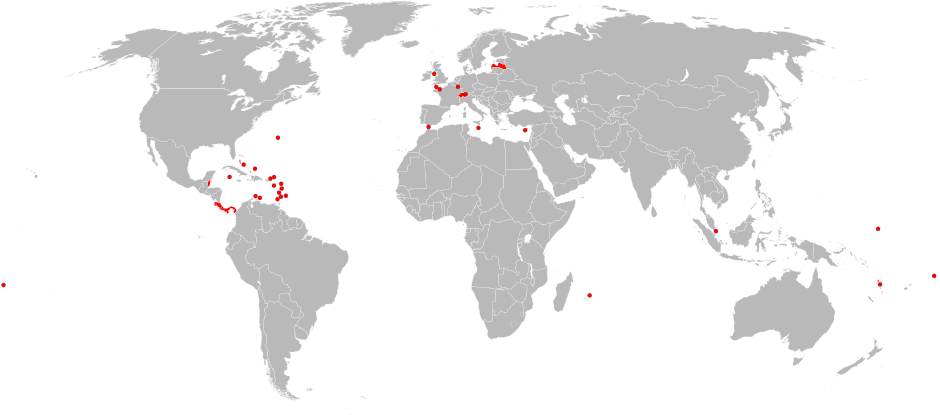
\includegraphics[scale=0.35]{img/taxhavens}
\end{frame}
\begin{frame}[allowframebreaks]{Main offshore financial centres and tax havens}
\begin{itemize}
\item
Bahamas, which has a considerable number of registered vessels. The Bahamas used to be the dominant force in the offshore financial world, but fell from favour in the 1970s after independence.
\item
Bermuda, which is market leader for captive insurance, and also has a strong presence in offshore funds and aircraft registration.
\item
British Virgin Islands, which has the largest number of offshore companies.
\item
Cayman Islands, which has the largest value of assets under management in offshore funds, and is also the strongest presence in the U.S. securitisation market.
\pagebreak
\item
Jersey has particularly strong banking and funds management sectors and a high concentration of professional advisers including lawyers and fund managers.
\item
Luxembourg, which is the market leader in Undertakings for Collective Investments in Transferable Securities (UCITS).
\item
Mauritius is used for both inward and outward investment platform for Asian, African and European countries, it has the effective commercial and legal infrastructure required to support the development of a global network. 
\pagebreak
\item
Panama, which is a significant international maritime centre. Although Panama (with Bermuda) was one of the earliest offshore corporate domiciles, Panama lost significance in the early 1990s.
\item
New Zealand, the remotest jurisdiction, has the advantage of being a true primary jurisdiction but with a tough but practical regulatory regime. It is well positioned for the Asian market but retains close ties to Europe.
\item
Dominica, which has the largest number of offshore companies formed in recent years. In recent years is now becoming a major financial center for offshore banks.
\item
Switzerland: taxes in Switzerland are levied by the Swiss Confederation, the cantons and the municipalities. Switzerland is sometimes considered a tax haven due to its general low rate of taxation, its political stability as well as the various tax exemptions or reductions available to Swiss companies doing business abroad, or foreign persons residing in Switzerland.
\end{itemize}
\end{frame}
\begin{frame}{The world`s five leading offshore finance centres}
\begin{itemize}
\item
Jersey
\item
Guernsey
\item
Isle of Man
\item
Bermuda Hamilton
\item
Cayman Islands
\end{itemize}
\end{frame}
\subsection{Offshore company management}
\begin{frame}{Offshore company management I}
\begin{itemize}[<+->]
\item
Option 1: Company directed by the beneficial owner. 
\item
Option 2: Company directed by an appointed Director (nominee). 
\end{itemize}
The owner of an offshore IBC may often be reluctant to publicly reveal his controlling position over a particular offshore company. 

If these considerations are important, the owner of the IBC, or any related individual who may be concerned with the same potential risks, should not be appointed to a direct managerial position of the offshore company. In this case, Company Management services (nominee services) should be chosen. 
\end{frame}
\begin{frame}[shrink=10]{Offshore company management II}
\begin{itemize}
\item
A professional Director ``rents out'' his name (``Nominee Director'').
\item
The owner may be formally appointed as the "representative" or "agent" of his IBC and sing himself all contracts, invoices and business correspondence.
\item
An active direct management of an IBC by the beneficial owner greatly reduces his level of personal secrecy in this respect (personal tax consequences for the owner).
\item
Comprehensive company management services provided by a third-party Director largely resolve the foreign taxation issue.
\item
Nominee shareholders. The professional service relationship between a Nominee Shareholder and the actual owner of the offshore company would usually be confirmed by a Trust Declaration
\end{itemize}
\end{frame}
\begin{frame}[shrink=10]{Business activities requiring special license}
\begin{itemize}
\item
    Trading in Foreign Exchange (Forex, FX)
\item
    Trading in financial commodity-based derivative instruments and other securities (futures, options, interest rates, shares, stock, contracts for differences etc.)
\item
    Money transmission services
\item
    Payment processing services
\item
    Money brokering
\item
    Money lending and pawning
\item
    Money exchange
\item
    Brokerage, consultancy and advisory services in any financial services
\item
    Accounting services
\item
    Safe custody services
\item
    International asset protection and management
\end{itemize}
\end{frame}
\begin{frame}{Benefits for registering financial services company in offshore}
\begin{itemize}[<+->]
\item
Tax exemption.
\item
Simple licensing requirements.
\item
Low level of regulations and simple documentary requirements 
\item
no obligation of financial reporting which allows the company to avoid complicated and expensive accountancy organization. 
\item
The only exception is the obligation to keep the minimum capital paid and unimpaired at all times. 
\end{itemize}
\end{frame}
\begin{frame}{The minimum paid-up capital requirements for financial services companies}
\begin{itemize}
\item
Trading in Foreign Exchange (Forex, FX) and other financial instruments (futures, options, interest rates, shares, stock, contracts for differences etc.) – USD~100~000.
\item
Money exchange – USD~75~000.
\item
Money transmission and payment processing services, money brokering, money lending and pawning – USD~50~000.
\item
Brokerage, consultancy and advisory services, safe custody services, accounting services, international asset protection and management – USD~25~000.

\end{itemize}
\end{frame}

\begin{frame}{The European Union withholding tax}
The European Union made a large number of offshore financial centres sign up to the European Union withholding tax. 

Under those regulations, brought into force by local law, banks in those jurisdictions which hold accounts for EU resident nationals must either deduct a 15\% withholding tax (which is split between the offshore jurisdiction and the country of the account holder`s residence), or permit full exchange of information with the country of the national`s residence.

A number of larger jurisdictions, including Hong~Kong and Singapore, refused to sign up to the directive.
\end{frame}
\end{document}